%%%%%%%%%%%%%%%%%%%%%%%%%%%%%%%%%%%%%%%%%
% Simple Sectioned Essay Template
% LaTeX Template
%
% This template has been downloaded from:
% http://www.latextemplates.com
%
% Note:
% The \lipsum[#] commands throughout this template generate dummy text
% to fill the template out. These commands should all be removed when 
% writing essay content.
%
%%%%%%%%%%%%%%%%%%%%%%%%%%%%%%%%%%%%%%%%%

%----------------------------------------------------------------------------------------
%	PACKAGES AND OTHER DOCUMENT CONFIGURATIONS
%----------------------------------------------------------------------------------------

\documentclass[12pt]{article} % Default font size is 12pt, it can be changed here

\usepackage{geometry} % Required to change the page size to A4
\geometry{a4paper} % Set the page size to be A4 as opposed to the default US Letter
\usepackage{listings}


\usepackage{graphicx} % Required for including pictures

\usepackage{float} % Allows putting an [H] in \begin{figure} to specify the exact location of the figure
\usepackage{wrapfig} % Allows in-line images such as the example fish picture

\usepackage{lipsum} % Used for inserting dummy 'Lorem ipsum' text into the template

\linespread{1.2} % Line spacing

%\setlength\parindent{0pt} % Uncomment to remove all indentation from paragraphs

\graphicspath{{Pictures/}} % Specifies the directory where pictures are stored

\begin{document}

%----------------------------------------------------------------------------------------
%	TITLE PAGE
%----------------------------------------------------------------------------------------

\begin{titlepage}

\newcommand{\HRule}{\rule{\linewidth}{0.5mm}} % Defines a new command for the horizontal lines, change thickness here

\center % Center everything on the page

\textsc{\LARGE University of Southampton}\\[1.5cm] % Name of your university/college
\textsc{\Large Threaded Programming Coursework}\\[0.5cm] % Major heading such as course name

\begin{minipage}{0.4\textwidth}
\emph{Author:}
Joshua Greenhalgh % Your name
\end{minipage}


{\large \today}\\[3cm] % Date, change the \today to a set date if you want to be precise

%\includegraphics{Logo}\\[1cm] % Include a department/university logo - this will require the graphicx package

\vfill % Fill the rest of the page with whitespace

\end{titlepage}

%----------------------------------------------------------------------------------------
%	TABLE OF CONTENTS
%----------------------------------------------------------------------------------------

\tableofcontents % Include a table of contents

\newpage % Begins the essay on a new page instead of on the same page as the table of contents 

%----------------------------------------------------------------------------------------
%	INTRODUCTION
%----------------------------------------------------------------------------------------

\section{Introduction} % Major section

This coursework will investigate various openmp loop scheduling options for a range of chunk sizes as well as describing a custom built loop schedule called affinity scheduling. The first section will outline the implementation of the in built openmp schedules applied to two different loops that where provided for this coursework - the schedule that gives the best performance for each loop will be selected and the effect of varying the number of threads will then be outlined. In the second section the construction of a custom scheduling method will be described and again the variation of the number of threads with respect to performance will be analysed for each of the two given loops.   
%------------------------------------------------

\section{Openmp Schedules} % Sub-section

Within openmp it is possible to automatically split the iterations of a for loop between threads, however this is only possible if each iteration is independent of all others - which is the case for the two loops we have been given. Each of the loop functions provided in \textit{loops.c} consist of two nested for loops, either of which could be parallelised but only the outermost loop has been. This is implemented using the following compiler directive placed just above the outermost loop;

\lstset{language=C}  % Start your code-block
\begin{lstlisting}
#pragma omp parallel for schedule(type [,chunk size])
\end{lstlisting}

This coursework will investigate the performance for the schedule types auto, static, dynamic and guided. All the schedule types, with the exception of auto, have the possibility of also defining a chunk size which will take values of $k = 1,2,4,8,16,32,64$. In order to discern the best schedule option the loops will be run on six threads initially - once the best schedule has been selected for each loop the number of threads will also be varied.

The static schedule attempts to divide the iterations into equal sized contiguous chunks and then shares these out to each thread as equally as possible at compile time. If the number of iterations is not divisible by the number of threads then it will not be possible for all chunks to be of equal size and so some chunks will be larger than others. If the optional chunk size argument is given then the compiler will split the iterations into chunks of the specified size.

Guided scheduling splits the loop into chunks of gradually decreasing size that are proportional to the number of iterations that remain. This causes the earlier chunks to be larger in size than the later ones. It is hoped that the earlier chunks are easier to compute however if this is not the case then it can be useful to reverse the direction of the iteration. Each of the chunks is assigned to a thread and when completed the thread is given a new chunk to process. The chunk size argument allows the user to define the minimum chunk size that will be used. 

The dynamic option is similar to static in that chunks are created to be as equal in size as possible. However rather than assigning each of the chunks to a particular thread at compile time the assignment is done at runtime as threads complete their block of iterations. This means that threads should be utilised as well as possible and will reduce the possibility of threads sitting idle that may occur when static is used.

The final schedule option is auto, this schedule is used mostly for loops that are run many times. This option allows the compiler to choose which schedule type to use initially and by collecting data on how the load is balanced each time the loop is run the schedule type will vary until the optimum schedule is found. 

\subsection{Data collection}

In order to collect data regarding the runtime for each schedule two bash scripts were created that made changes to two C template files. The first script \textit{schedulescript} modifies the file \textit{schedule.c} by inserting each of the schedule options and creating a series of new C files one for each schedule option. Each of these files is then compiled and run with the output data printed to stdout which can then be directed to a text file to store the results. The second script \textit{threadscript} modifies the file \textit{threads.c} again creating a series of new C files for each of the thread numbers ($t = 1,2,3,6,12,24$), each of these C files is then compiled and run with results printed to stdout. The file \textit{threads.c} has the best schedule option for each loop hard coded the only variation is in the number of threads used.  

The compilation of the C files was undertaken using the GNU compiler using -o3 flag in order to optimise the code as much as possible. The executable files were run on the login node of Archer.

\subsection{Loop 1}

\begin{figure}[H] % Example image
\center{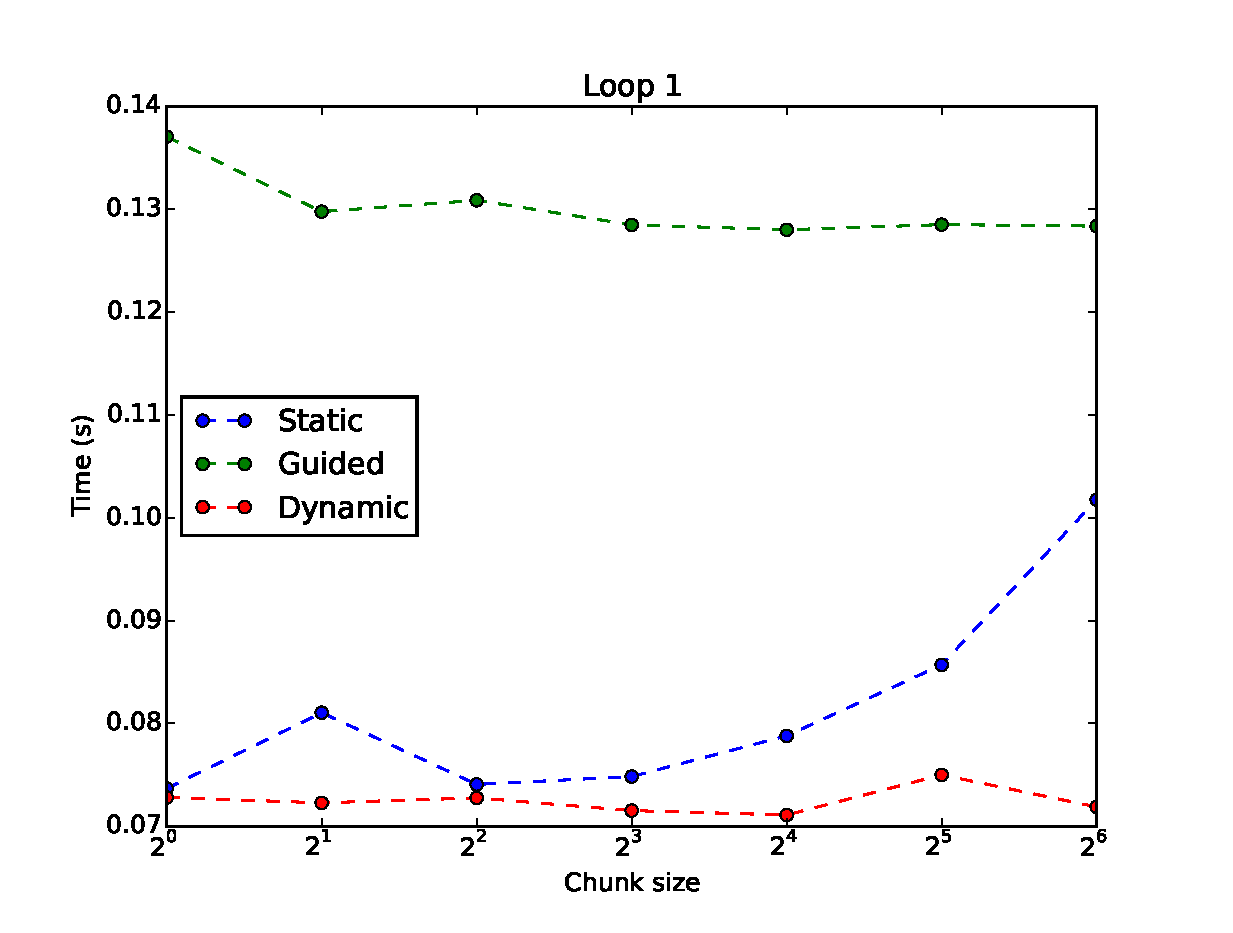
\includegraphics[width=\linewidth]{loop1}}
\caption{The loop 1 runtimes for the schedules static, guided and dynamic with varying chunk size options}
\label{fig:speciation}
\end{figure}

As can be seen from the above figure the dynamic schedule was quickest for all chunk sizes with little variation. The guided schedule was slowest for all chunk sizes again with little variation after the chunk size was increased from one . Static schedules show a marked increase in runtime as chunk size is increased. The following table shows the quickest runtimes for each schedule. 

\begin{center}
    \begin{tabular}{| l | l | l | l | l | l |}
    \hline
    schedule &static,1 & static &dynamic,16 & guided,16 & auto \\ \hline
    time (s) &0.073682&0.128575 & 0.0711& 0.127999& 0.128213\\ \hline
    \end{tabular}
\end{center} 

The best schedule for loop 1 is dynamic with a chunk size of 16, this will be used to investigate the effect of varying the number of threads.

\subsection{Loop 2}

\begin{figure}[H] % Example image
\center{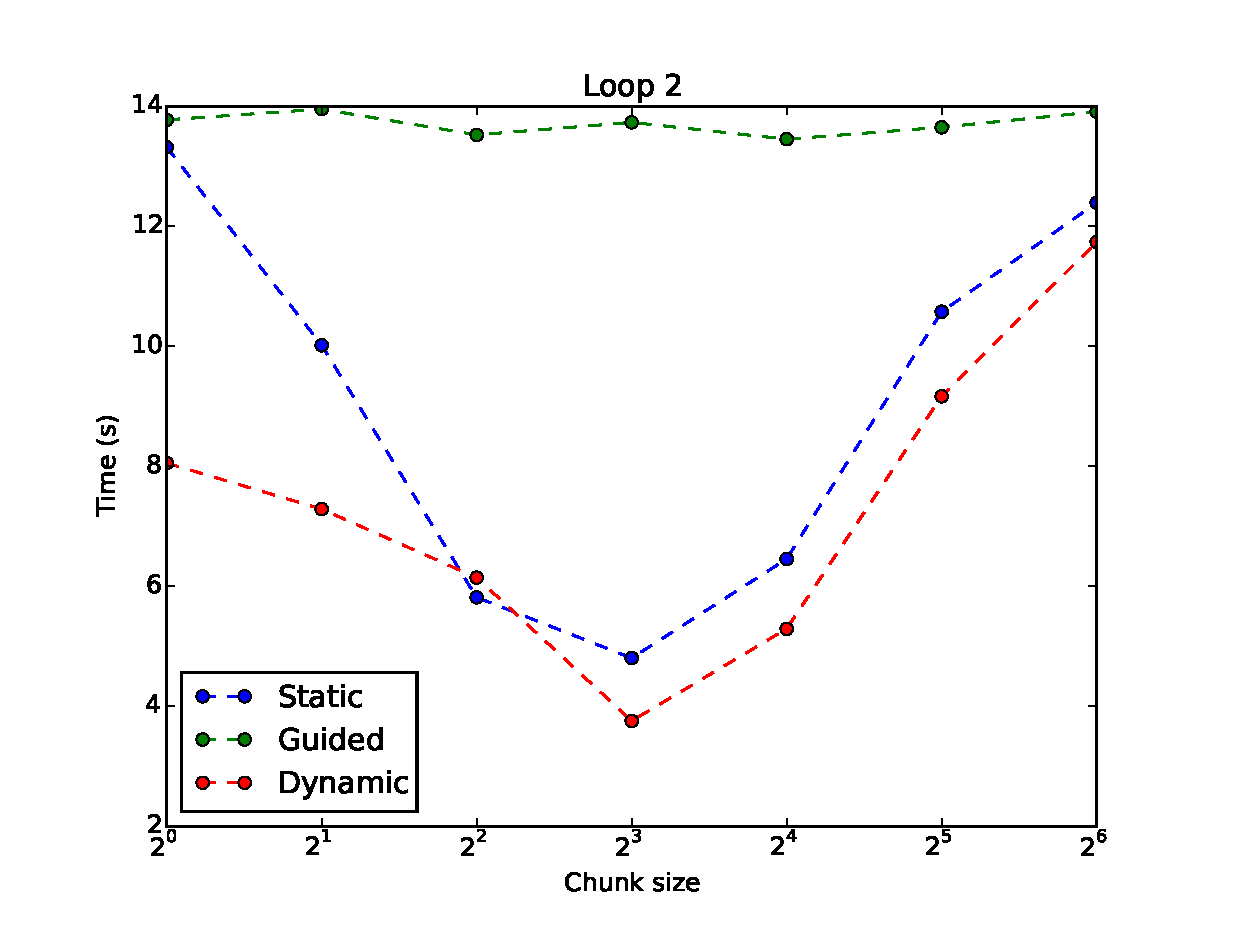
\includegraphics[width=\linewidth]{loop2}}
\caption{The loop 2 runtimes for the schedules static, guided and dynamic with varying chunk size options}
\label{fig:speciation}
\end{figure}

It is clear that this loop is much more computational intensive than loop 1 as can be seen from the runtimes in the above figure. As was the case in loop 1 the guided schedule was the slowest of the three and took a fairly consistent time to run regardless of the chunk size used. Both static and dynamic schedules show parabolic trend in run time as chunk size is increased with a minimum run time when a chunk size of 8 is used, however dynamic schedule is generally quicker than static other than the at a chunk size of 4. The following table shows the quickest runtimes for each schedule. 

\begin{center}
    \begin{tabular}{| l | l | l | l | l | l |}
    \hline
    schedule &static,8 & static &dynamic,8 & guided,16 & auto \\ \hline
    time (s) &4.804029&13.642967 & 3.757006& 13.452082& 13.662151\\ \hline
    \end{tabular}
\end{center} 

The quickest schedule option for loop 2 is dynamic with a chunk size of 8, again this schedule will be used to investigate variation in the number of threads.

\subsection{Variation of number of threads}
 
\begin{figure}[H] % Example image
\center{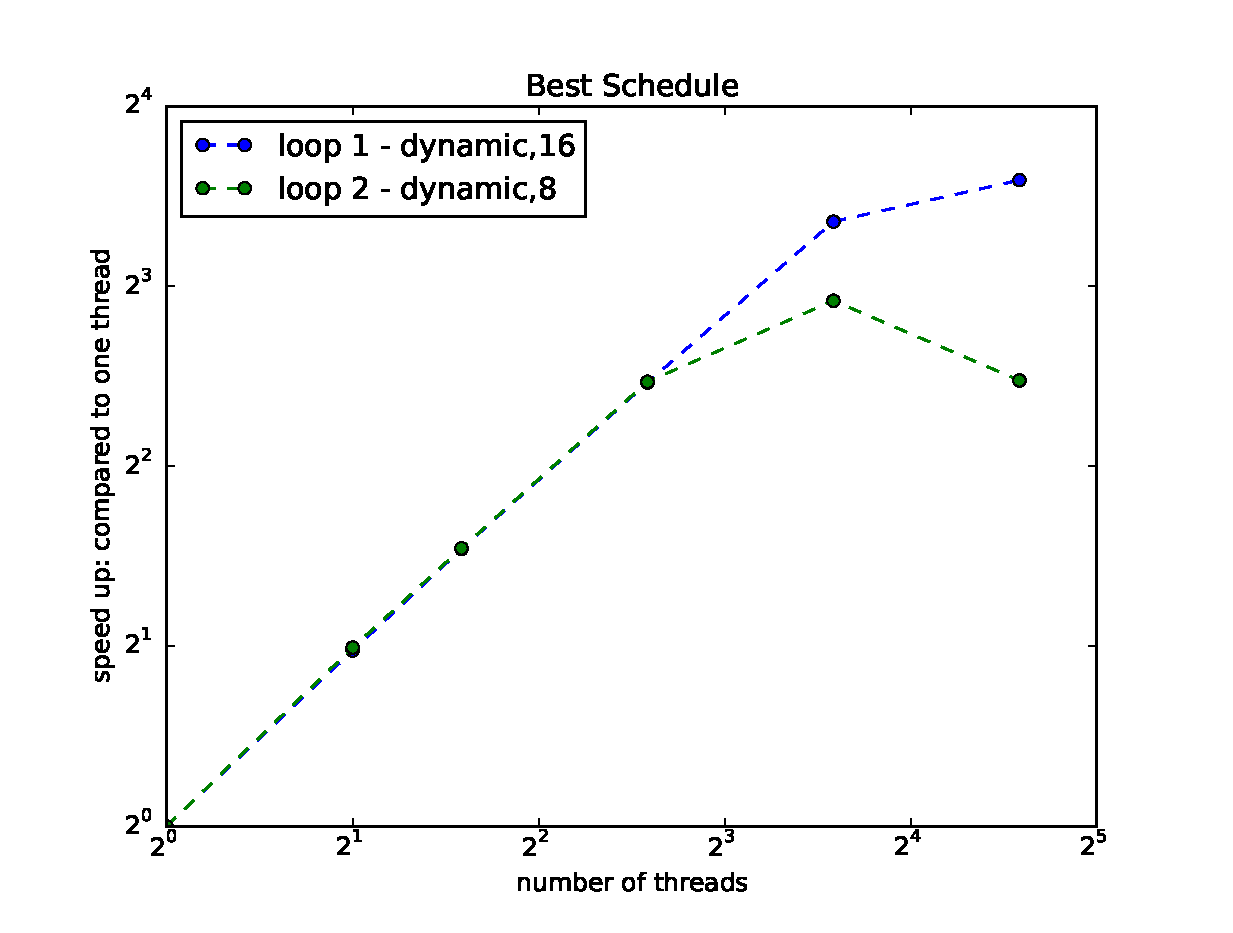
\includegraphics[width=\linewidth]{BestSchedules}}
\caption{Loglog plot of the speedup gained by increasing the number of threads}
\label{fig:speciation}
\end{figure}

Both loop 1 and loop 2 where run for various numbers of threads using the best schedules found in the previous sections. By calculating the speed up in comparison to the base case of using one thread it is clearly seen that there is a linear increase in speed until around 6 threads. At this point the loop 1 speed continues to increase but not as quickly, however loop2 begins to slow down once 24 threads are used. 


%------------------------------------------------

\section{Affinity Schedule} % Sub-section

The affinity schedule splits the set of iterations into a contiguous local set of iterations one for each of the $P$ threads. Each local set is of size $\frac{n}{P}$, where $n$ is the total number of iterations. If $n \bmod P$ is not equal to zero then a single extra iteration is distributed to the threads $p = 0,..,(n \bmod P) - 1$. The local sets are then divided into chunks of decreasing size which are proportional to the number of iterations in the local set that have not been yet been placed in a chunk. Each thread should process its own local set of iterations beginning with its largest assigned chunk. When a thread has depleted all the chunks it has been assigned then it should begin to process chunks from other the threads local sets beginning with the largest chunk currently available.

The implementation I have created is based on a set of FIFO queue structures, one for each thread. Each queue is able to add elements to its rear, remove elements from the front and is also able to view without removing elements from the front. The insertion and removal of elements is possible in a single operation since the queue structure maintains a pointer to the memory location of both its front and rear elements. Elements within the queue are themselves data structures which contain three integer fields; the start iteration of a chunk, the end iteration and the size of the chunk.

The algorithm proceeds in two main sections;

\begin{enumerate}
  \item Distribution of the local sets to each thread via the creation of a populated queue containing the chunks in decreasing order of size.
  \item Processing each threads local set of iterations followed by the processing of other threads chunks if any are available.  
  \end{enumerate}
  
  
 \subsection{Distribution of chunks and creation of queues}
 
The distribution of chunks is undertaken in the functions; \textit{construct\_global\_partition} and \textit{partition\_localset}. The first of these functions determines the upper and lower bounds of the local sets for each thread. These are stored in an array of size $P+1$ such that the first and second elements are the upper and lower bounds for thread zero, the second and third for thread one, etc. This array is then passed to the function \textit{partition\_localset}, which is run in a parallel region, along with an array of pointers to memory allocated for each threads queue structure. Each thread then initialises its queue structure ,by assigning null pointers to its rear and front, before populating with its local chunks.  
 
 \subsection{Processing of iterations}
 
The processing of iterations is performed by the functions; \textit{process\_own\_Ql1}, \textit{process\_own\_Ql2}, \textit{process\_other\_Qsl1} and \textit{process\_other\_Qsl2} - the l1 and l2 variants of these functions simply call different versions of the loop function which was provided. The function \textit{process\_own\_Q} successively removes the front element from its own queue and passes the data structure to the loop function to perform the iterations. Upon completion of a threads own queue it begins to run the function \textit{process\_other\_Qs}. This function, with the help of another function \textit{nxt\_chunk}, loops over each of the other threads queues looking at, but not removing, the top element in order to find the remaining chunk of largest size. When the largest available chunk has been found it is only then removed from the queue and passed to the loop function to perform the iterations this is repeated until all threads queues are empty. In order to avoid race conditions the removal of elements from the queues is conducted within a critical region - this protects against the possibility of two threads attempting to remove the same queue element and means that it is not possible for a chunk to be processed multiple times.  

It should be noted that my implementation does not repeat the set of iterations one hundred times as in the preceding section, the loop is only run a single time. It should be possible to change the code so that this can be achieved however on completion of the loop each queue is empty and would need to be repopulated which may significantly slow the implementation down.   

\subsection{Results}
\begin{figure}[H] % Example image
\center{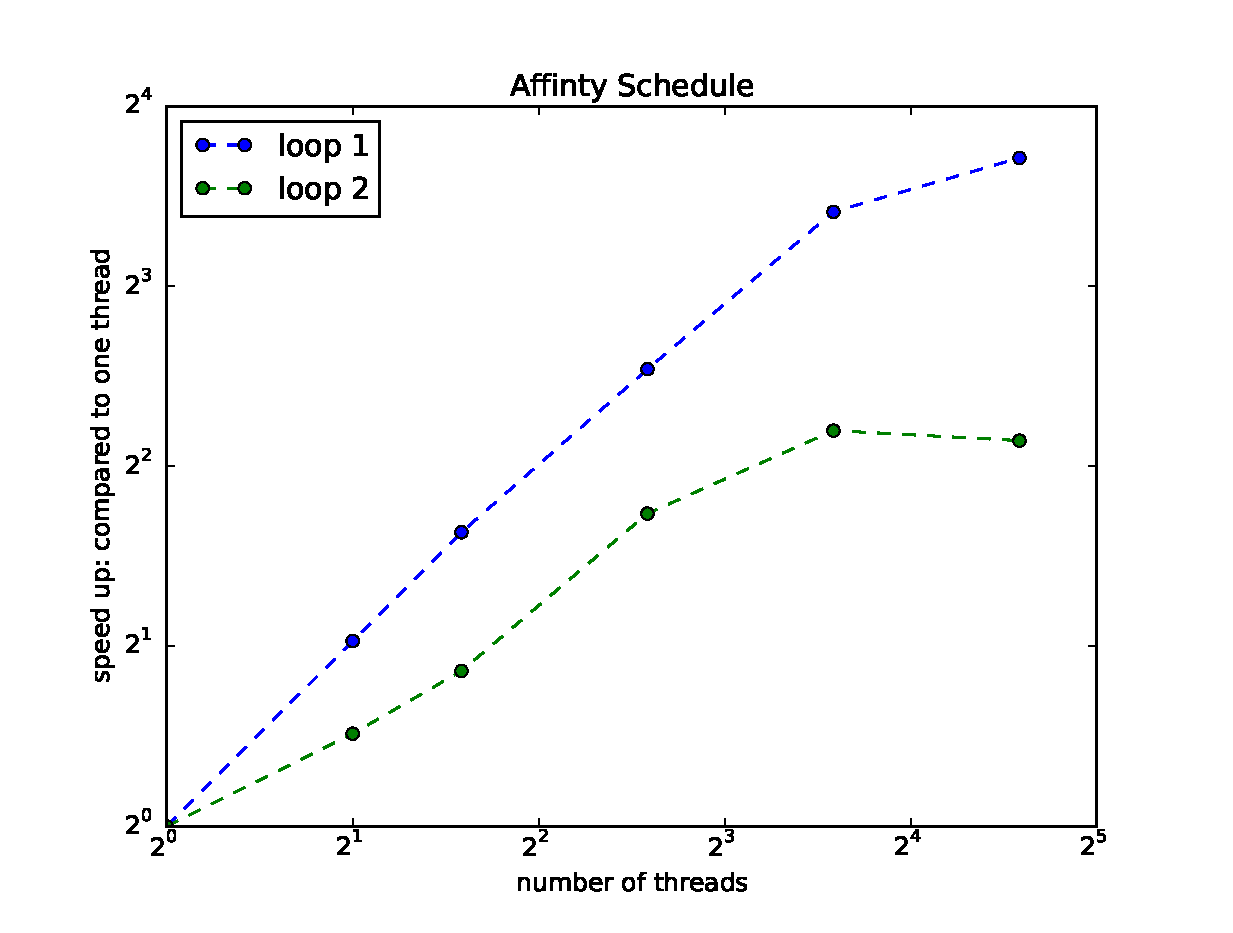
\includegraphics[width=\linewidth]{AffintySchedule}}
\caption{Loglog plot of the speedup gained by increasing the number of threads}
\label{fig:speciation}
\end{figure}

As can be seen from the above figure this implementations runtime scales linearly with increase of threads up until around 12 threads. The increase in speed for loop 1 is linear with gradient of approximately one whereas loop 2 is linear but with a smaller gradient. It also clear that loop 2 begins to see a drop off in speed when 24 threads are used whereas loop 1 continues to increase in speed. 


\begin{figure}[H] % Example image
\center{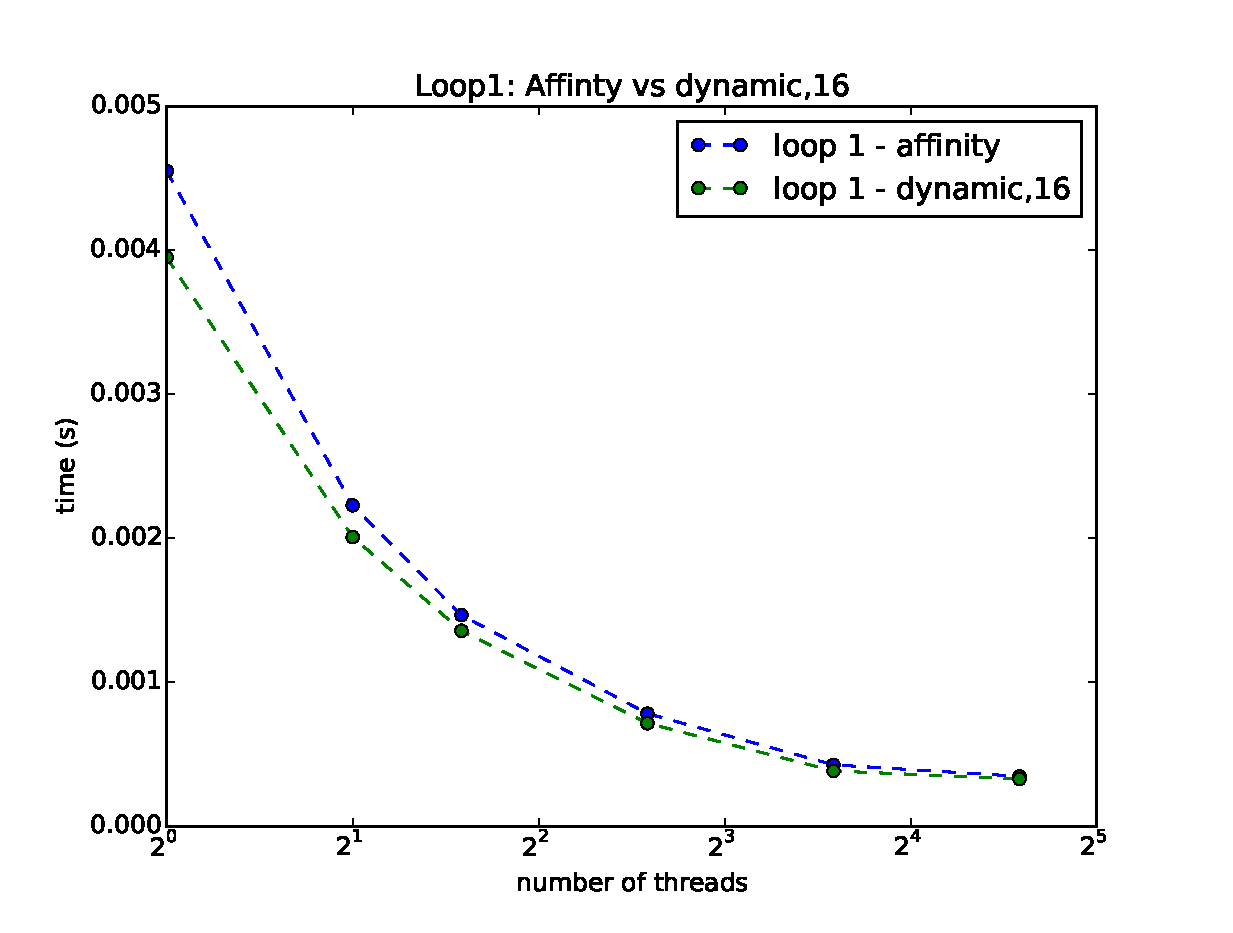
\includegraphics[width=\linewidth]{L1afvdyn16}}
\caption{runtime for loop1}
\label{fig:speciation}
\end{figure}

The above figure shows the actual runtimes for loop 1 using the best built in schedule (dynamic,16) as well as my implementation of affinity scheduling. Since my implementation only ran the loop a single time the runtime for dynamic has been averaged by dividing by the 100 repetitions. For this loop my implementation compares well with the in built schedule, it is generally slightly slower however as the number of threads increases the two schedules begin to show almost identical performance. In figure 6 the actual runtimes are shown for loop 2 - again my implementation is showing  that it compares well with the best schedule found for this loop. The difference in runtime for this loop, between my implementation and the in built openmp schedule, stays approximately the same regardless of the number of threads in contrast to the results seen for loop 1.

\begin{figure}[H] % Example image
\center{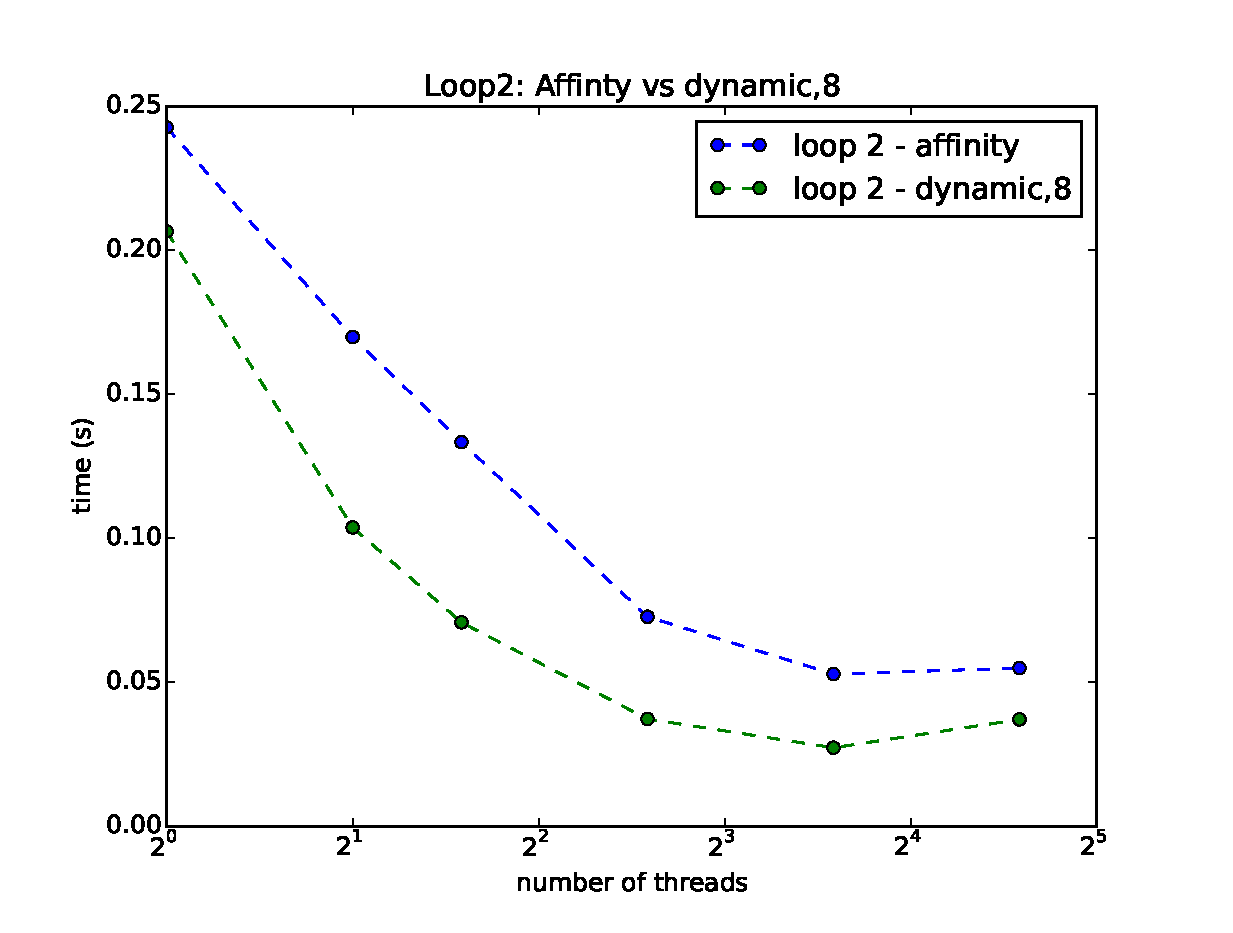
\includegraphics[width=\linewidth]{L2afvdyn8}}
\caption{runtime for loop2}
\label{fig:speciation}
\end{figure}

%------------------------------------------------


%----------------------------------------------------------------------------------------
%	MAJOR SECTION X - TEMPLATE - UNCOMMENT AND FILL IN
%----------------------------------------------------------------------------------------

%\section{Content Section}

%\subsection{Subsection 1} % Sub-section

% Content

%------------------------------------------------

%\subsection{Subsection 2} % Sub-section

% Content

%----------------------------------------------------------------------------------------
%	CONCLUSION
%----------------------------------------------------------------------------------------


\end{document}